\documentclass[a4]{scrartcl}
\usepackage[utf8]{inputenc}
\usepackage{hyperref}
\usepackage{color}
\usepackage{tikz}
\usepackage{pgf}
\usepackage{graphicx}
\usepackage{amsmath, amssymb}
\usepackage{pdfpages}

\newcommand\invisiblesection[1]{%
  \refstepcounter{section}%
  \addcontentsline{toc}{section}{\protect\numberline{\thesection}#1}%
  \sectionmark{#1}}

\begin{document}

\author{Simon Schlepphorst \and Federico Diaz Capriles}
\title{Ising Model}
\subtitle{A Statistical System at Finite Temperature}
\date{16 March 2017}

\maketitle

\begin{abstract}
	This paper explores a two dimensional Ising model by the use of Markov
	Chain Monte Carlo (MCMC). Two algorithms, Metropolis-Hastings and
	Swendsen-Wang, are described and used to simulate a lattice,
	demonstrate phase transitions from the Ising model, and shows the
	effect of temperature on the magnetization of a lattice. Furthermore,
	this paper compares both algorithms in terms of efficiency and
	limitations. Lastly, initial conditions of the lattice (hot, cold or
	random) are discussed.
\end{abstract}

\tableofcontents

\section{Theory}

	\begin{minipage}{.6\textwidth}
		\centering
		
\begin{tikzpicture}
			\draw[step=.5cm,gray,very thin] (0.1,0.1) grid (2.9,2.9);
			\fill[black] (0.1,0.1) rectangle (.5,1.5);
			\fill[black] (0.1,1.5) rectangle (2,2);
			\fill[black] (2,0.1) rectangle (2.5,0.5);
			\fill[black] (1.5,0.5) rectangle (2,1);
			\fill[black] (0.5,1) rectangle (1,1.5);
			\fill[black] (2,2) rectangle (2.9,2.9);
		\end{tikzpicture}
		\captionof{figure}{Example for a spin lattice}
		\label{fig:ising}
	\end{minipage}%
	\begin{minipage}[]{.4\textwidth}
		$ \square $ Spin up \\ 
		$ \blacksquare $ Spin down 
	\end{minipage}

%TODO Insert a caption for this figure. Minipage doesnt allow \caption 

\subsection{Introduction to the Ising Model}
The ising model is a mathematical model of a lattice by use of statistical
mechanics. The lattice is modeled by a  $ n \times m $ matrix of which each
element takes a value of $+1$ or $-1$. Each element now represents a particle
or atom within the lattice and this value is its spin or magnetic moment. This
model can be used to identify properties of a lattice such as phase transition
temperatures, magnetization, specific heat, etc.

Consider figure~\ref{fig:ising} to be a representation of our $ n \times m $ matrix. The
Hamiltonian that describes this kind of lattice is given by eq.~\eqref{eq:ham}

\begin{equation} \label{eq:ham}
\mathcal{H}(\textbf{s}) = - \sum_{\langle i, j \rangle} J_{ij} s_{i} s_{j} -
	\mu \sum_{j} h_j s_j
\end{equation}
{\scriptsize \begin{equation*}
s_{n} \in \{-1,+1\}
\end{equation*}}\vspace{-.5cm}
\begin{equation*}
\textbf{s} = (s_{1}, s_{2}, \dots, s_{N})
\end{equation*}
 
Where J is an interaction parameter that gives how site $ j $ interacts with
its near neighbors ($ i $), $\mu$ is the magnetic moment, $h_j$ is an external
magnetic field interacting with site $ j $, and \textbf{s} is a spin
configuration where each $s_n$ is the spin orientation of site $n$. For a
positive J value we have ferromagnetic interaction between sites $ j $ and $ i
$. Meaning that all spins will want to be aligned within the lattice. Negative
J values denote antiferromagnetic interactions and therefore spins will want to
be opposite to its neighbors.

If we take our lattice to not be under the influence of an external field and
assume that the interaction between any two sites is the same throughout the
lattice we can simplify our Hamiltonian as follows:
 
\begin{equation}
\mathcal{H}(\textbf{s}) = -J \sum_{\langle i, j \rangle} s_{i} s_{j}
\end{equation}

Because we have a thermodynamic system, we know the configuration probability $
\mathcal{P} $ is given by the Boltzmann distribution (eq.~\eqref{eq:bolz}) and
canonical partition function (eq.~\eqref{eq:canpar}):

\begin{equation}\label{eq:bolz}
	\mathcal{P}(\textbf{s}) = \frac{e^{-\beta \mathcal{H}(\textbf{s})}}
		{\mathcal{Z}}
\end{equation}
{\scriptsize \begin{equation*}
	\beta \equiv \frac{1}{k_{B} T}
\end{equation*}}

\begin{equation}\label{eq:canpar}
\mathcal{Z} = \sum_{\textbf{s}} exp(-\beta \mathcal{H}(s))
\end{equation}

Regarding statistics, for a lattice of L total sites and two possible spin
values per site we get $2^{L}$ potential configurations. This is very difficult
to do by hand and so Monte Carlo methods will be implemented in the simulation
of lattices and property analysis.
	
\subsection{Markov Chains}

\begin{figure}[h!]
	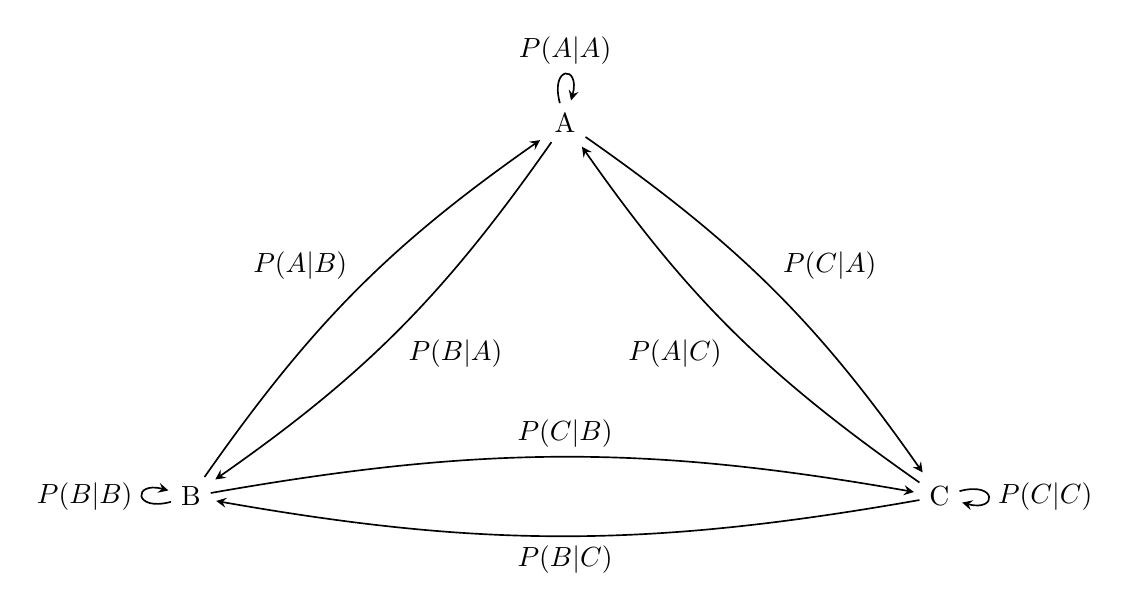
\begin{tikzpicture}[->,>=stealth,shorten >=2pt,auto,node distance=5cm,
	semithick]
	
	\tikzstyle{every state}=[fill=black,draw=none,text=white]
	
	\node        (A)                     {A};
	\node        (B) [below left=4.5cm]  {B};
	\node        (C) [below right=4.5cm] {C};
	
	\path (A) edge [loop above] node {${P(A | A)}$} (A)
	edge [bend left=10] node {${P(B| A)}$} (B)                    
	edge [bend left=10] node {${P(C| A)}$} (C)
	(B) edge [loop left]  node {${P(B| B)}$} (B)
	edge [bend left=10] node {${P(C| B)}$} (C)
	edge [bend left=10] node {${P(A| B)}$} (A)
	(C) edge [loop right] node {${P(C| C)}$} (C)
	edge [bend left=10] node {${P(A| C)}$} (A)
	edge [bend left=10] node {${P(B| C)}$} (B);
	\end{tikzpicture}\caption{A diagram of a simple Markov chain}
\end{figure}

A Markov chain is a mathematical system that allows us to jump from one state
to another via some probability. In Fig.2, we can see a brief description of a
Markov chain where each letters denotes a state. In parallel to the project at
hand, one can see that A, B and C are just lattice configurations. Of course it
is important to note that a physical system will have states with probability
to remain as they are or change. Furthermore, a Markov chain is "memoryless."
That is to say, a Markov chain only cares for the possible states it can go to
and the current state it is in regardless of what state came before.

Markov chains are useful because they allow us to generate directly from a
given distribution ($\pi$) like a Boltzmann distribution in this example.

The tool that lets us jump from some initial state $\mu$ to some final state
$\nu$ is called a transition matrix $P$. This matrix is exemplified in the
following matrix:
\[
P = 
\begin{bmatrix}
P_{11} & P_{12} & P_{13} &    \dots    & P_{1m} \\
P_{21} & P_{22} & P_{23} &    \dots    & P_{2m} \\
\vdots & \vdots & \vdots & P_{\mu \nu} & \vdots \\
P_{n1} & P_{n2} & P_{n3} &    \dots    & P_{nm}
\end{bmatrix}\] 

This transition matrix has very nice properties that give us the ability to
sample from our wanted distribution:
\begin{description}
	\item[Irreducibility:] Every state can be reached from any other state in a final number of steps.
	\item[Positive Recurrent:] The chain returns to $\mu$ from $\mu$ in a finite time
	\item[Detailed Balance:] $ \pi_\mu P_{\mu \nu} = \pi_\nu P_{\nu \mu} $
\end{description}
Detailed balance also introduces a new label for our distribution $\pi$. It can
now be called an invariant distribution which has the following properties by
definition:
\begin{description}
	\item[Invariant Distribution:] If $\pi$ and $P$ are in detailed balance and $\pi$ is a stationary distribution of $P$ then $\pi = \pi P$
	\item[Stationary Distribution:] $\pi_\mu$ must exists for all states $\mu$, is independent of the initial state, and $ \sum_\mu \pi_\mu = 1 $. 
\end{description}

All these properties allow us to use Markov chains to simulate a lattice and
see how the states transition.
\subsection{Markov Chains Monte Carlo}
	

\section{Metropolis-Hastings Algorithm}
\subsection{Algorithm}

\subsection{Results}

\subsection{Problems and Limitations}

\section{Swendsen-Wang Algorithm}
\subsection{Algorithm}

\subsection{Results}
\pageref{MCT}

\subsection{Problems and Limitations}

\appendix
\invisiblesection{Metropolis-Hastings Algorithm}
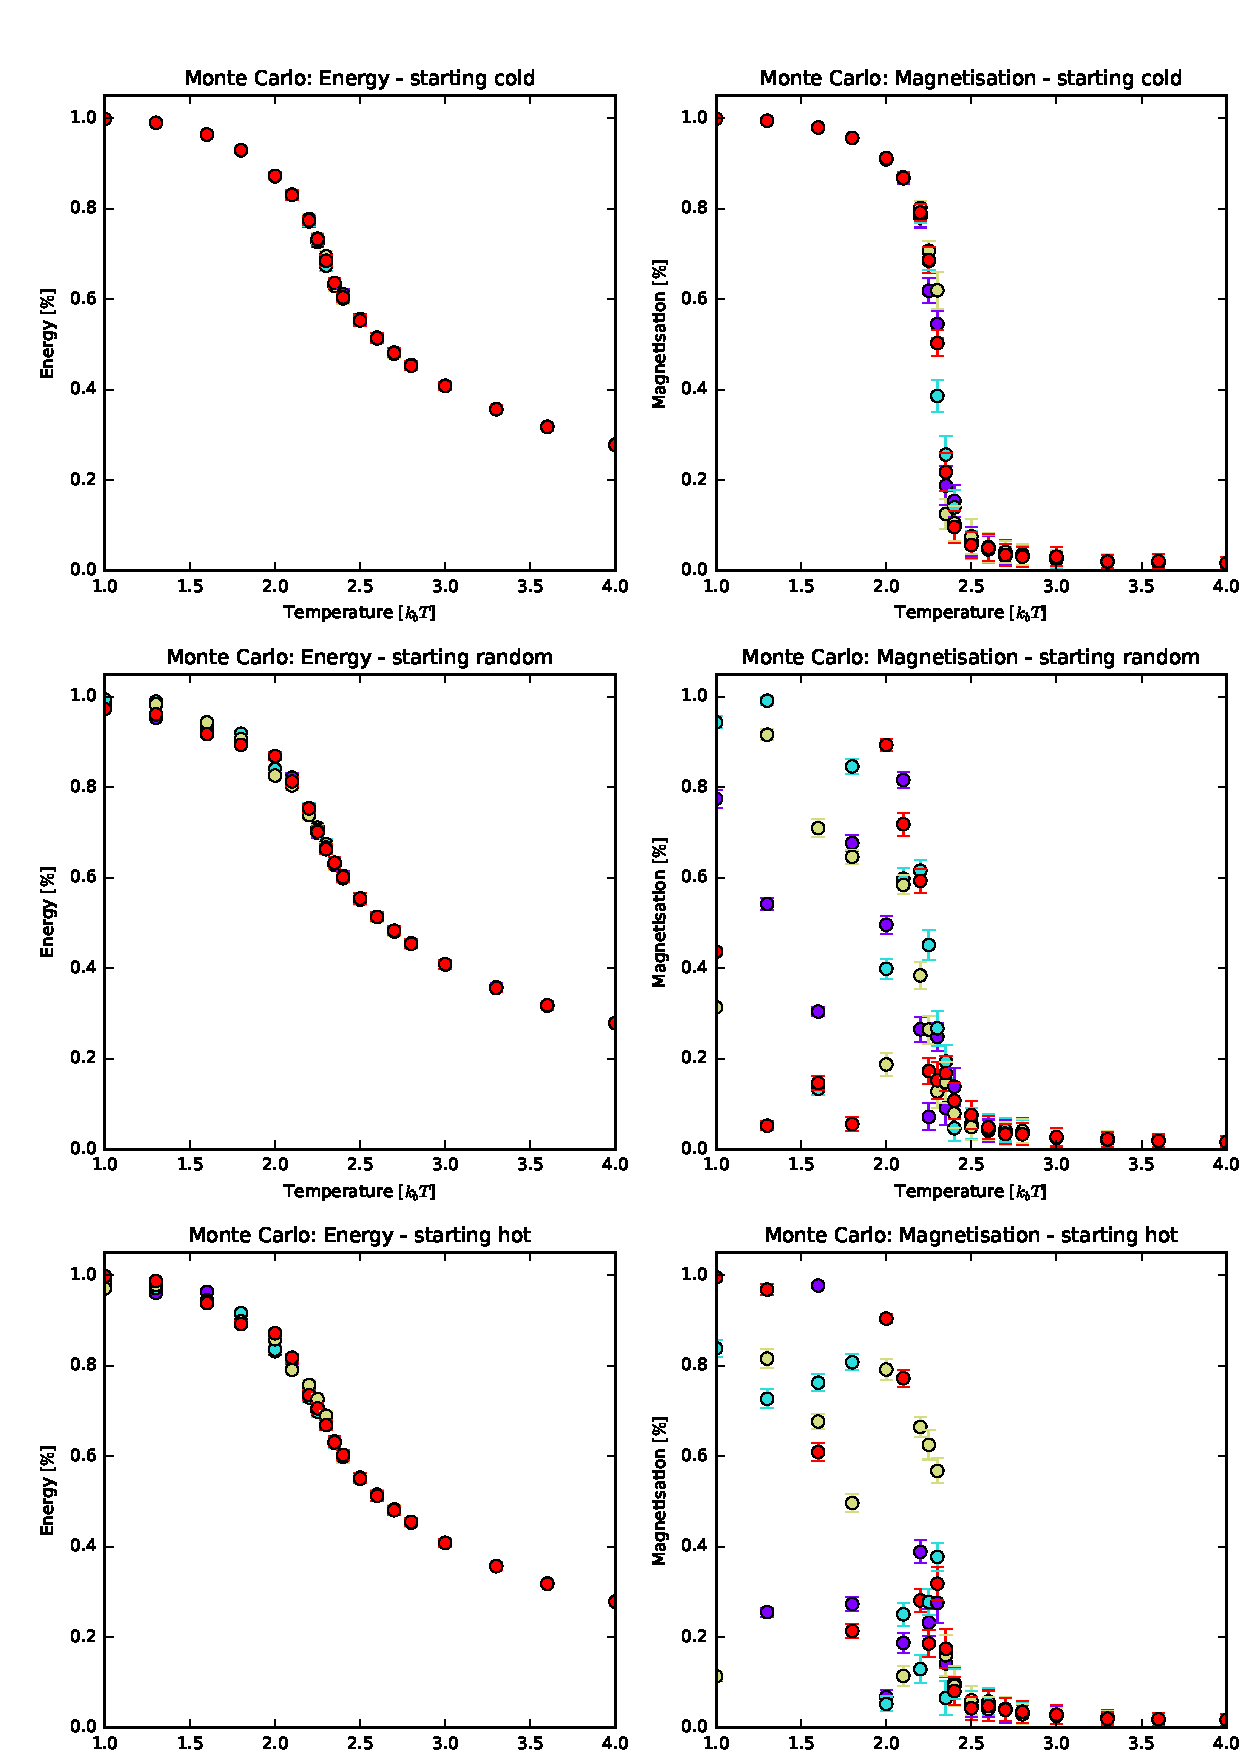
\includepdf[pages={-}, addtotoc={1,subsection,2,Temperature,MCT}, scale=0.9]{_build/Monte-Carlo_Temperatures.pdf}
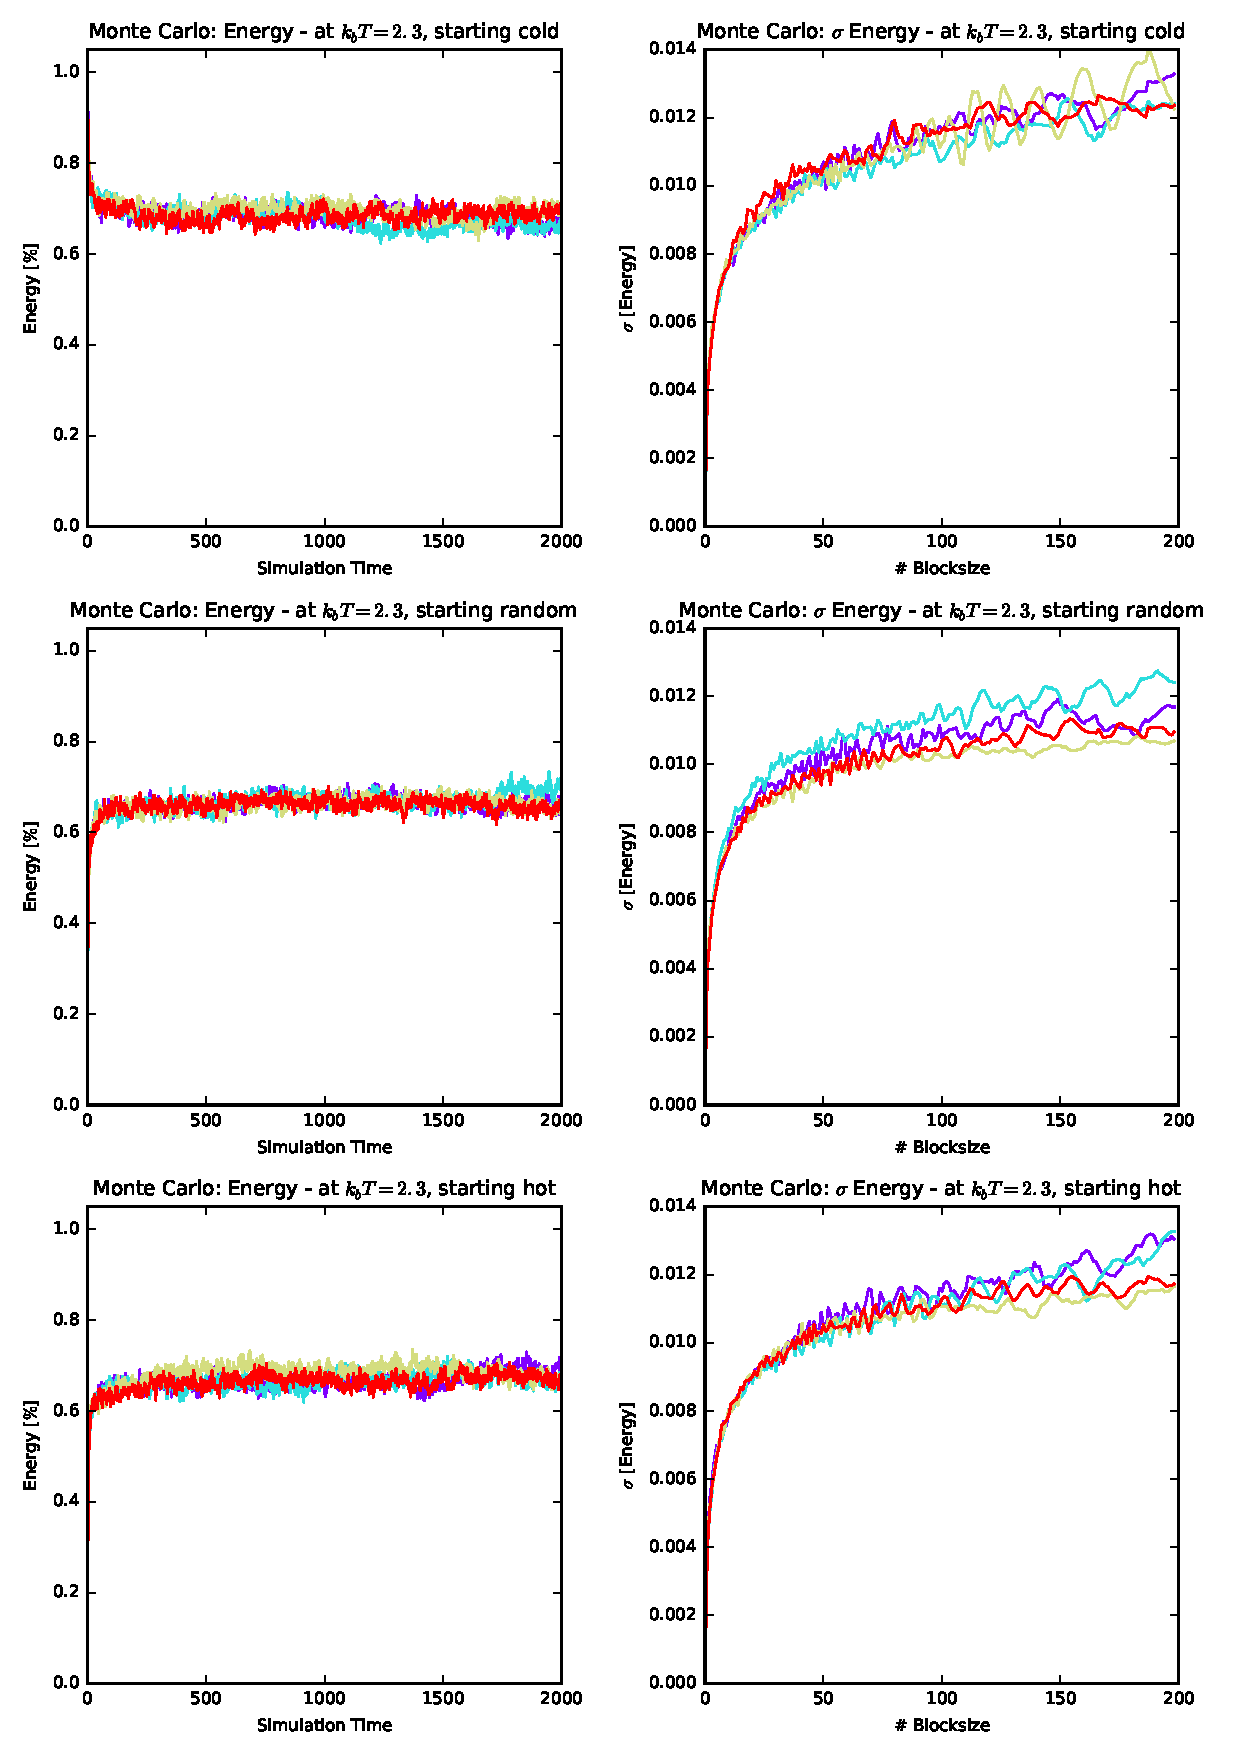
\includepdf[pages={-}, addtotoc={1,subsection,2,Energy,MCE}, scale=0.9]{_build/Monte-Carlo_Energy.pdf}
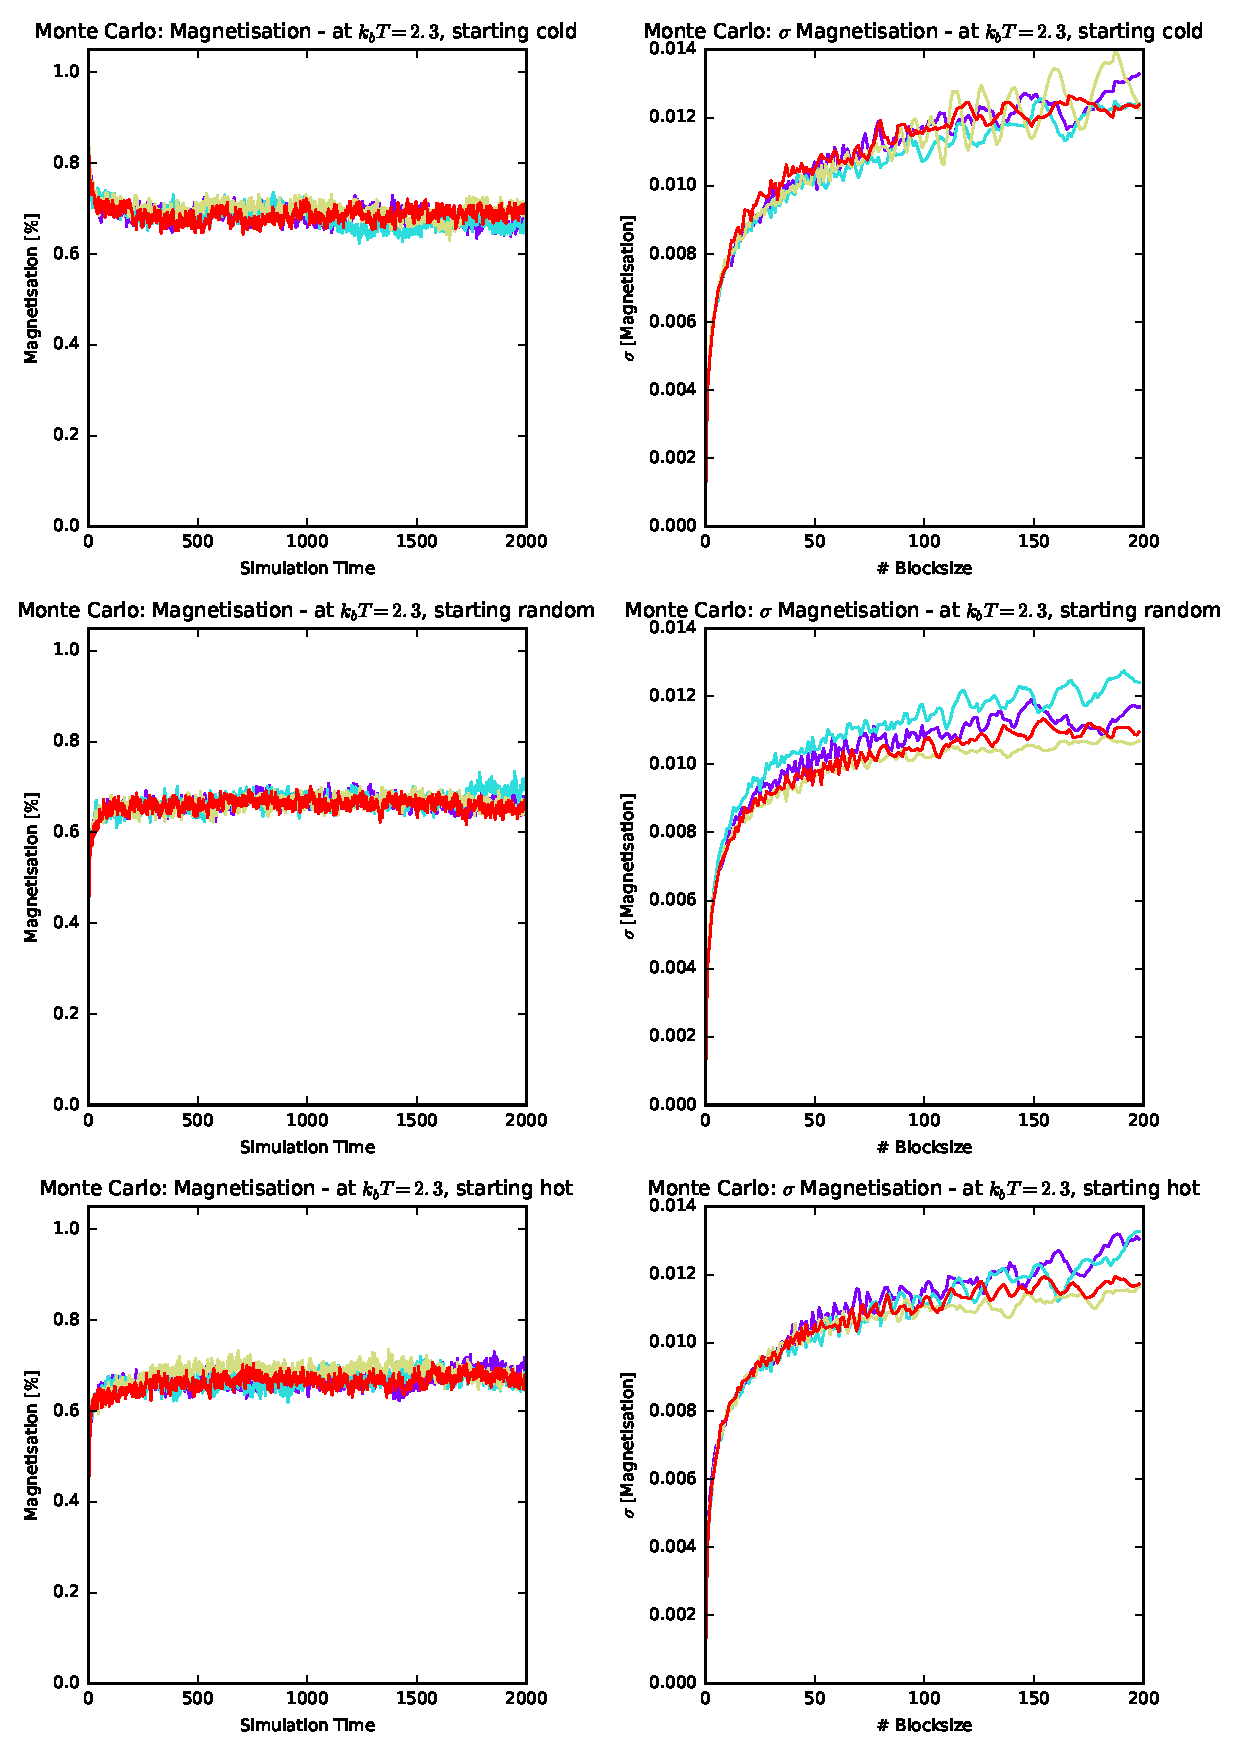
\includepdf[pages={-}, addtotoc={1,subsection,2,Magnetisation,MCM}, scale=0.9]{_build/Monte-Carlo_Magnetisation.pdf}

\invisiblesection{Cluster Agorithm}
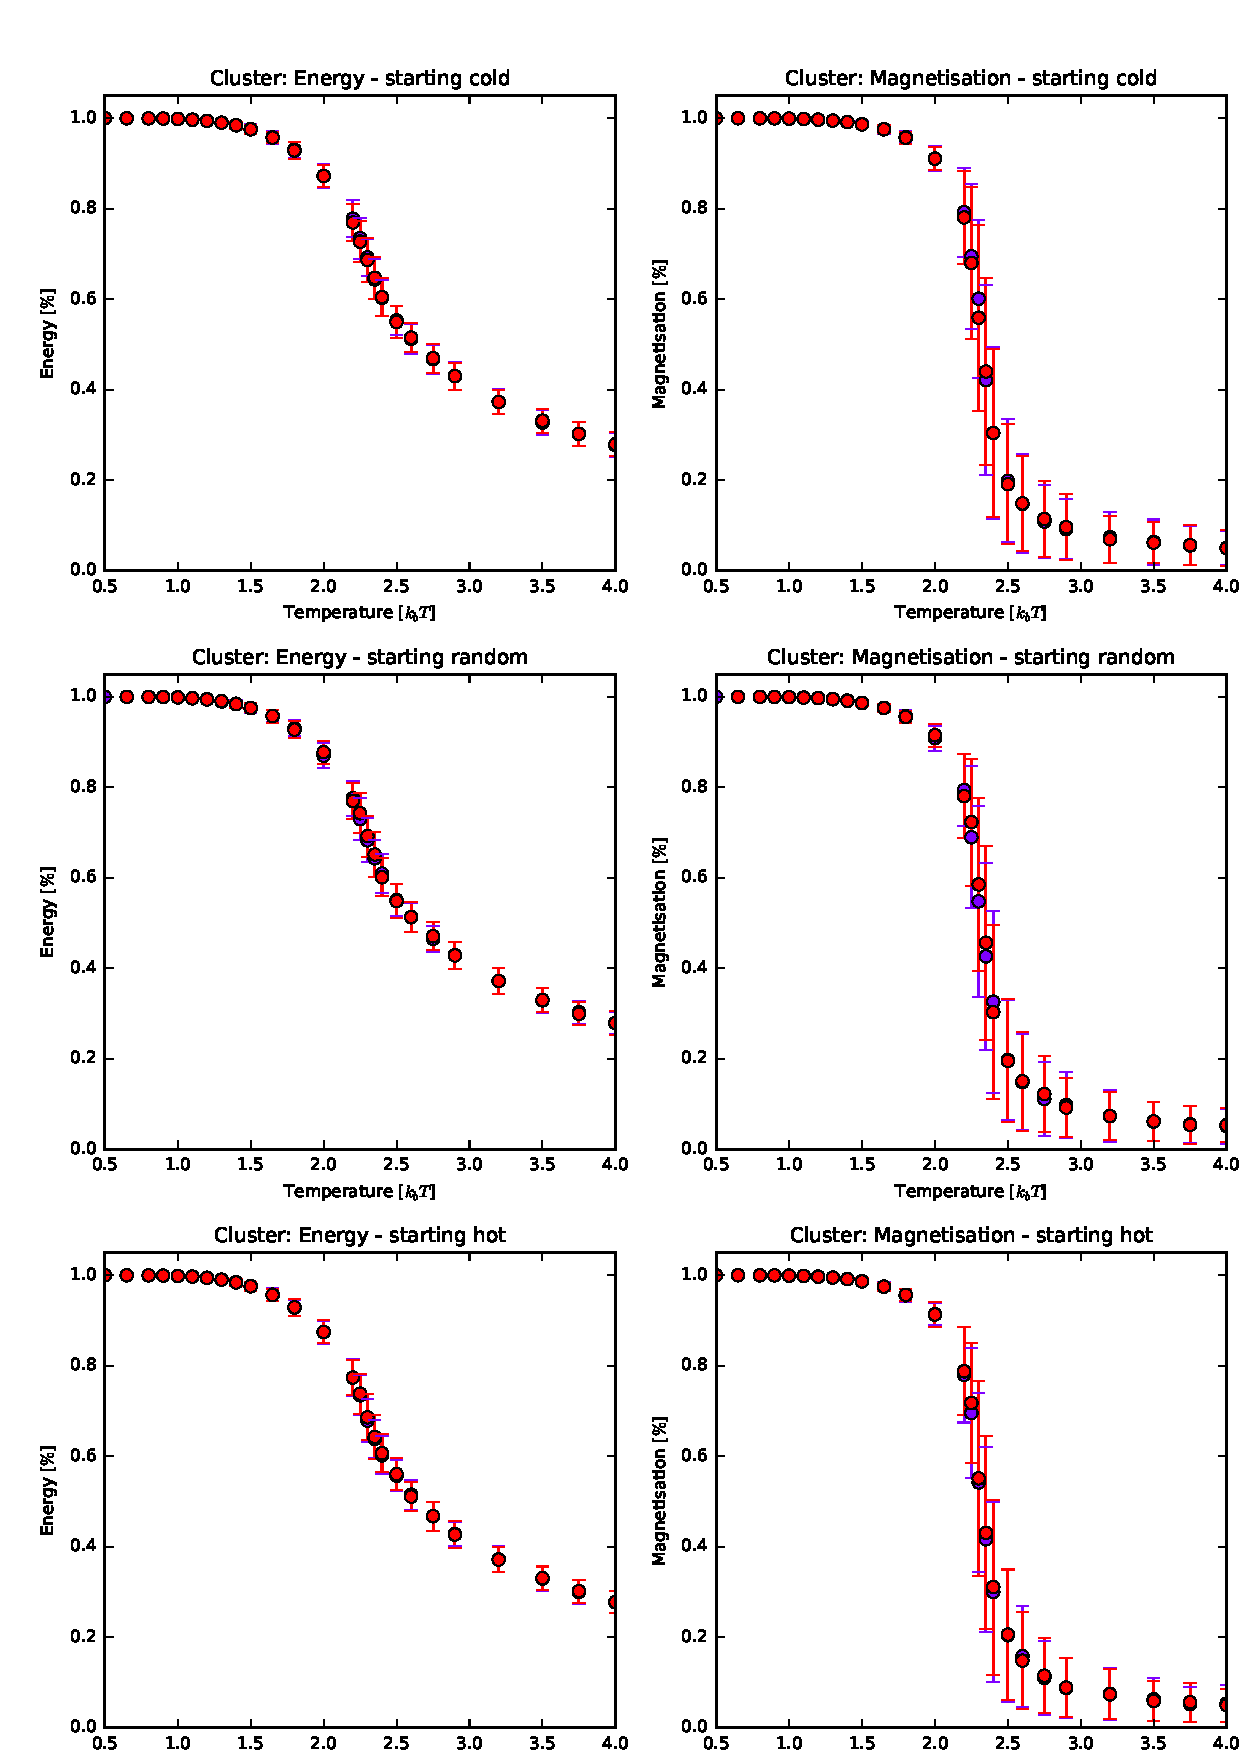
\includepdf[pages={-}, addtotoc={1,subsection,2,Temperature,CLT}, scale=0.9]{_build/Cluster_Temperatures.pdf}
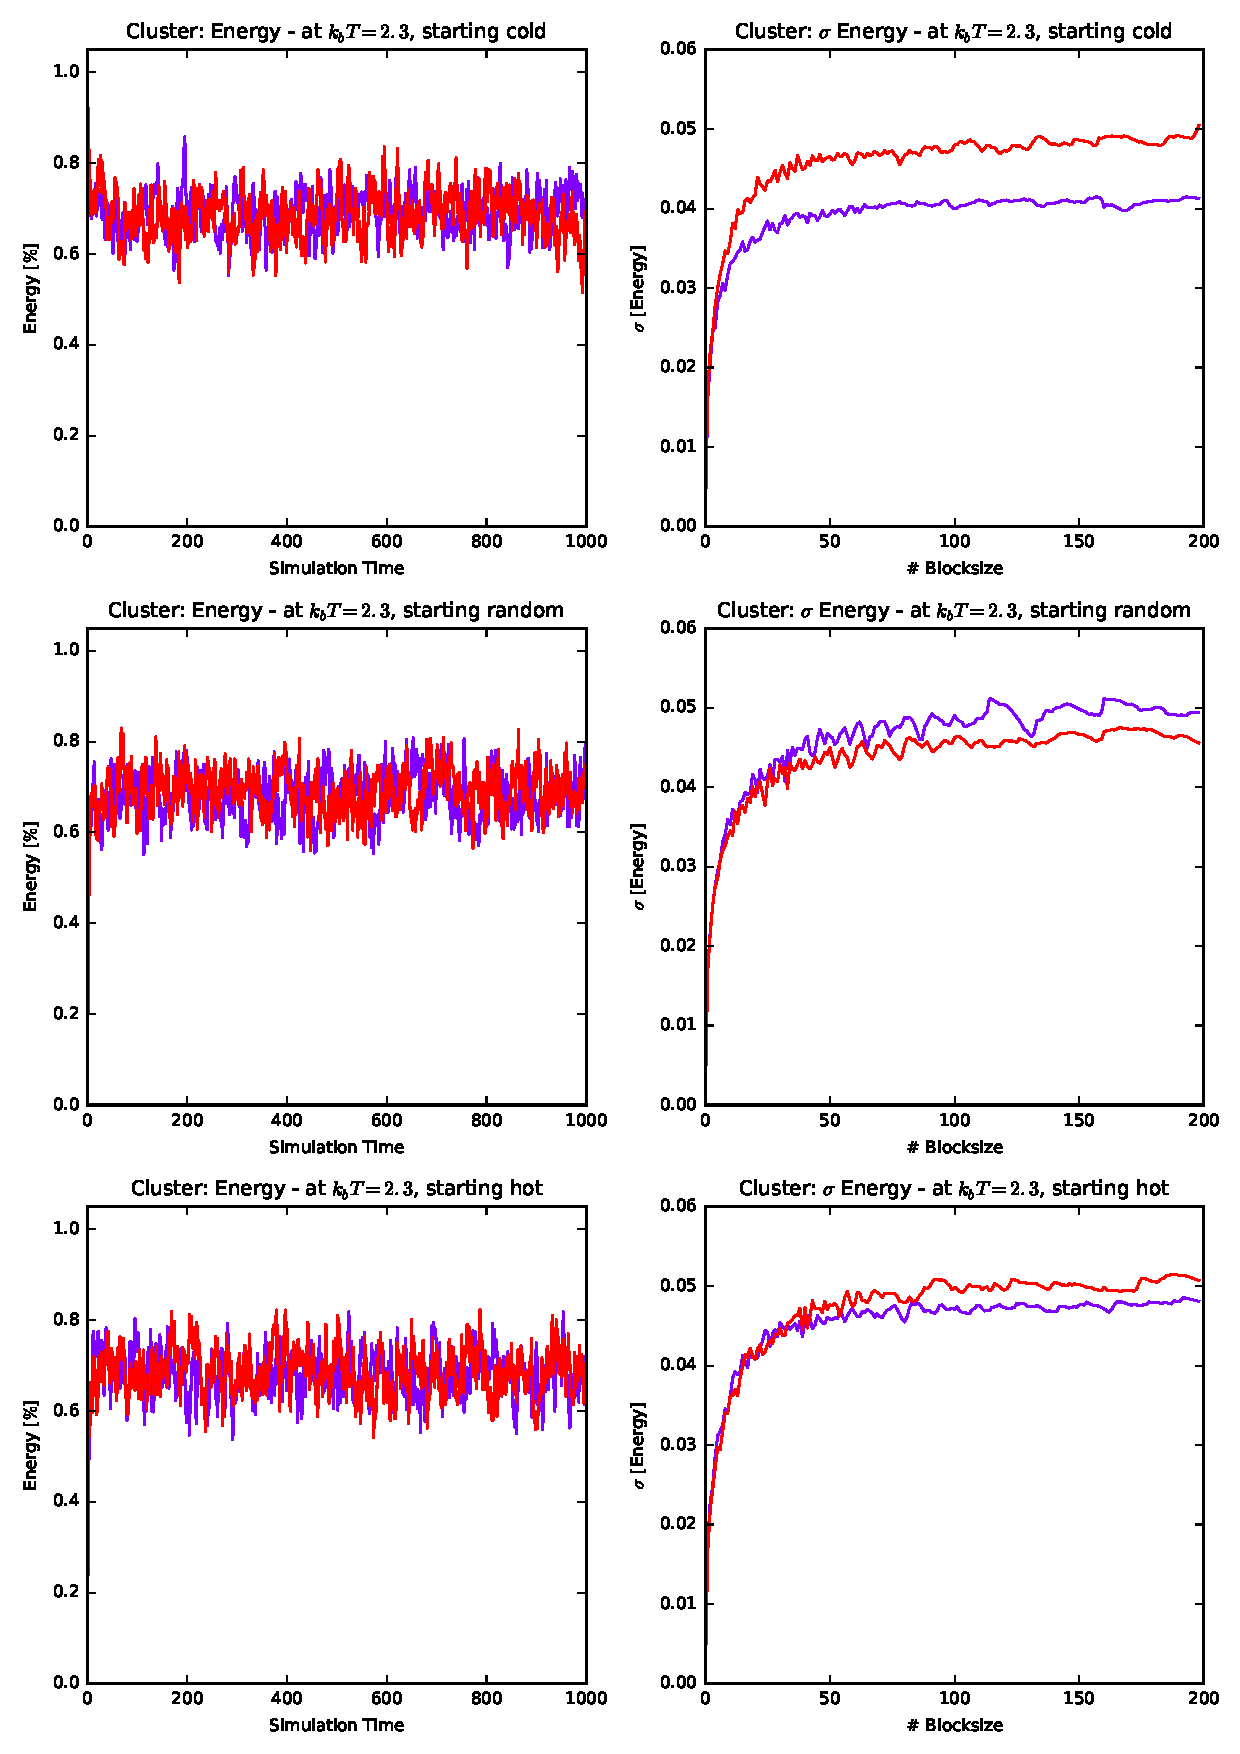
\includepdf[pages={-}, addtotoc={1,subsection,2,Energy,CLE}, scale=0.9]{_build/Cluster_Energy.pdf}
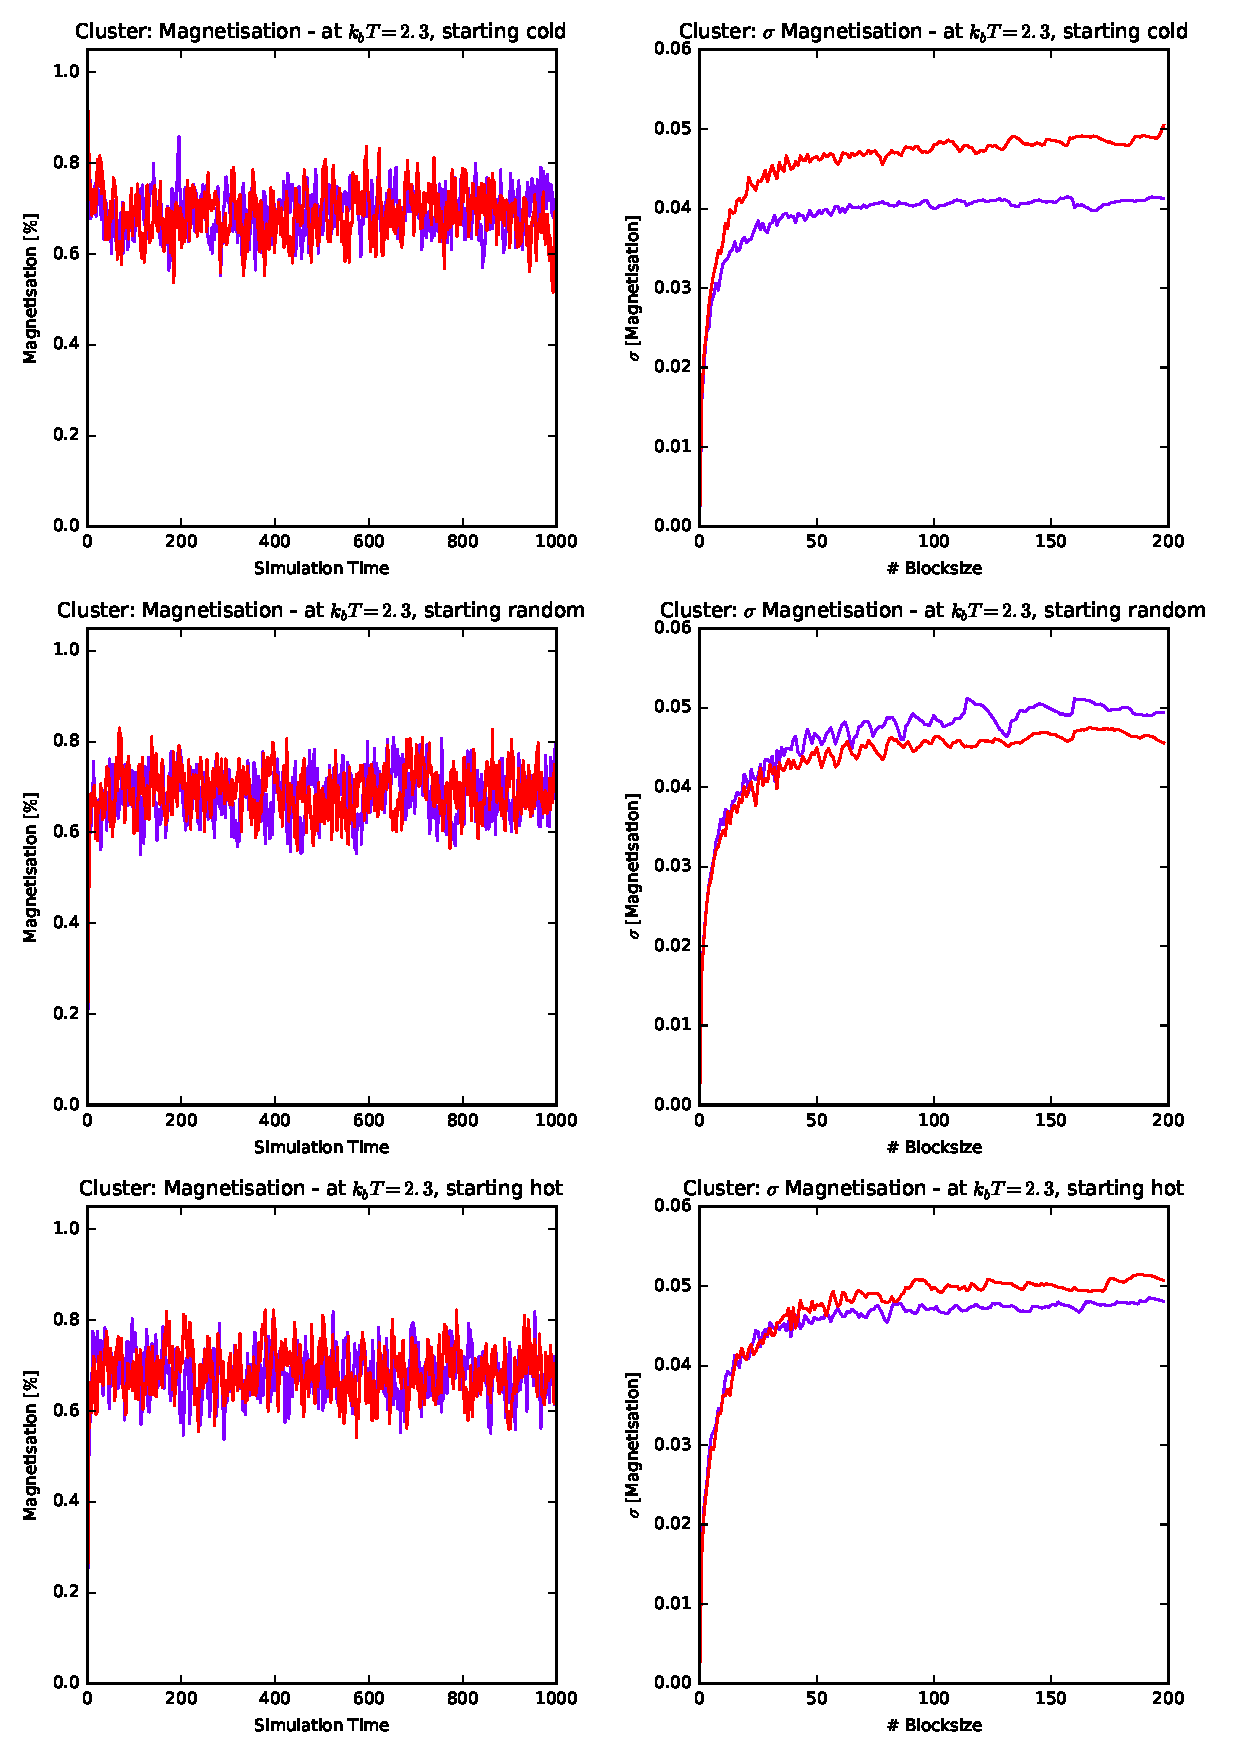
\includepdf[pages={-}, addtotoc={1,subsection,2,Magnetisation,CLM}, scale=0.9]{_build/Cluster_Magnetisation.pdf}

\end{document}
